\documentclass[svgnames]{beamer}
\mode<presentation>
\usefonttheme{serif}
\usecolortheme{dove}
\useinnertheme{rounded}
%\useoutertheme{smoothbars}
\setbeamercolor{item projected}{fg=black}
\setbeamertemplate{navigation symbols}{}

\usepackage{times}
\usepackage[french]{babel}
\usepackage{amsthm,amssymb,amsmath,graphicx}
\usepackage{color}
\usepackage{gastex}
\usepackage{framed}
\usepackage{graphicx}
\usepackage{multicol}
\usepackage{ulem}
\usepackage{ifthen}
\usepackage{tikz}

%%%%%%%%%%%%%%%%%%%%%%%%%%%%%%%%%%%%%%%%%%%%%%%%%%%%%%%%%%%%%%%%%%%%%%%%%%%%%%%%%%%%%%%%
%%%%%%%%%%%%%%%%%%%% A non-original creation by Nathanaël Fijalkow and Victor Marsault %

\setbeamertemplate{frametitle}{
  \vskip-2pt
  \begin{beamercolorbox}[rightskip=2cm,leftskip=1em,dp=1ex,wd=12.8cm]{frametitle}
    \vskip2pt
    \usebeamercolor{frametitle}
    \begin{tikzpicture}
      \useasboundingbox (0,0) rectangle (0,0); 
      \ifthenelse{\insertframenumber<\inserttotalframenumber}
      { 
        \pgfmathsetmacro{\aimangle}{90-(\insertframenumber*360/\inserttotalframenumber)}
        \fill [fill=frametitle.fg,thin, color=gray!50,draw=black] (11.8,.2) -- (11.8,.6) arc (90:\aimangle:0.4) -- cycle;

      }{ 
        \fill[fill=frametitle.fg,thin, color=gray!50,draw=black] (11.8,0.2) circle (.4);
      }
      \fill[fill=frametitle.fg,thin, color=white,draw=black] (11.8,0.2) circle (.3);
      \node at (11.8, .2) [black,circle]{\normalsize\insertframenumber};
    \end{tikzpicture}
    \insertframetitle
    \vskip2pt
  \end{beamercolorbox}
}
%%%%%%%%%%%%%%%%%%%%%%%%%%%%%%%%%%%%%%%%%%%%%%%%%%%%%%%%%%%%%%%%%%%%%%%%%%%%%%%%%%%%%%%

\setbeamertemplate{blocks}[rounded]
\setbeamercolor{block title}{bg=normal text.bg!90!black}
\setbeamercolor{block body}{bg=normal text.bg!95!black}

\newcommand{\A}{\mathcal{A}}
\newcommand{\Q}{\mathbb{Q}}
\newcommand{\N}{\mathbb{N}}
\newcommand{\tr}[1]{\langle #1 \rangle}
\newcommand{\prob}[1]{\mathbb{P}_{#1}}
\newcommand{\set}[1]{\{ #1 \}}
\newcommand{\val}[1]{\text{val}(#1)}

  
\title{CNRS Concours 06/03}
\subtitle{Nathana{\"e}l Fijalkow}
\institute{University of Oxford}
\date{}

\begin{document}

\addtocounter{framenumber}{-1}

\begin{frame}
  \titlepage
\end{frame}

\begin{frame}{Parcours}
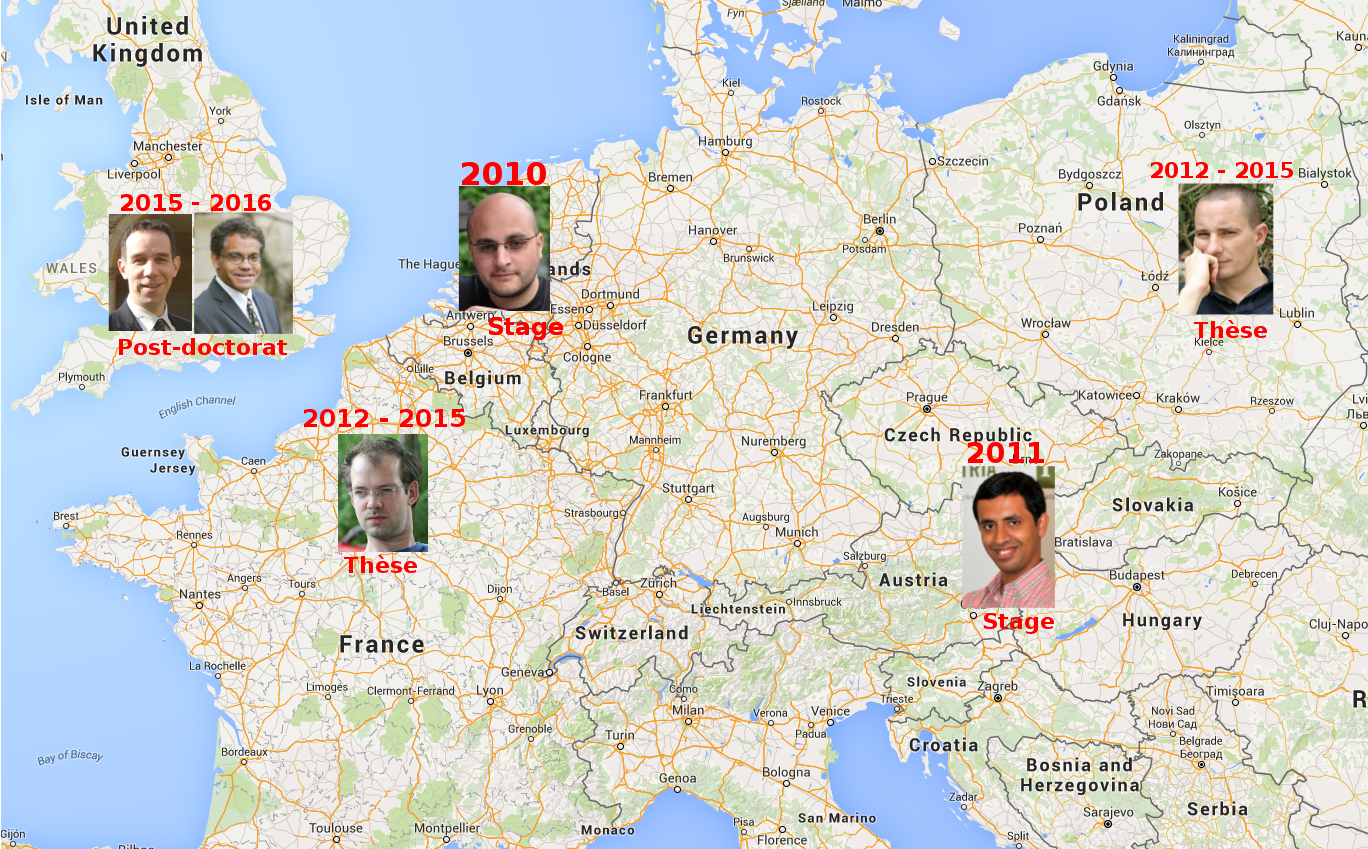
\includegraphics[width=11cm]{Fig/Europe_pic_tag}
\end{frame}

\begin{frame}{Coauteurs (articles sans mes encadrants)}
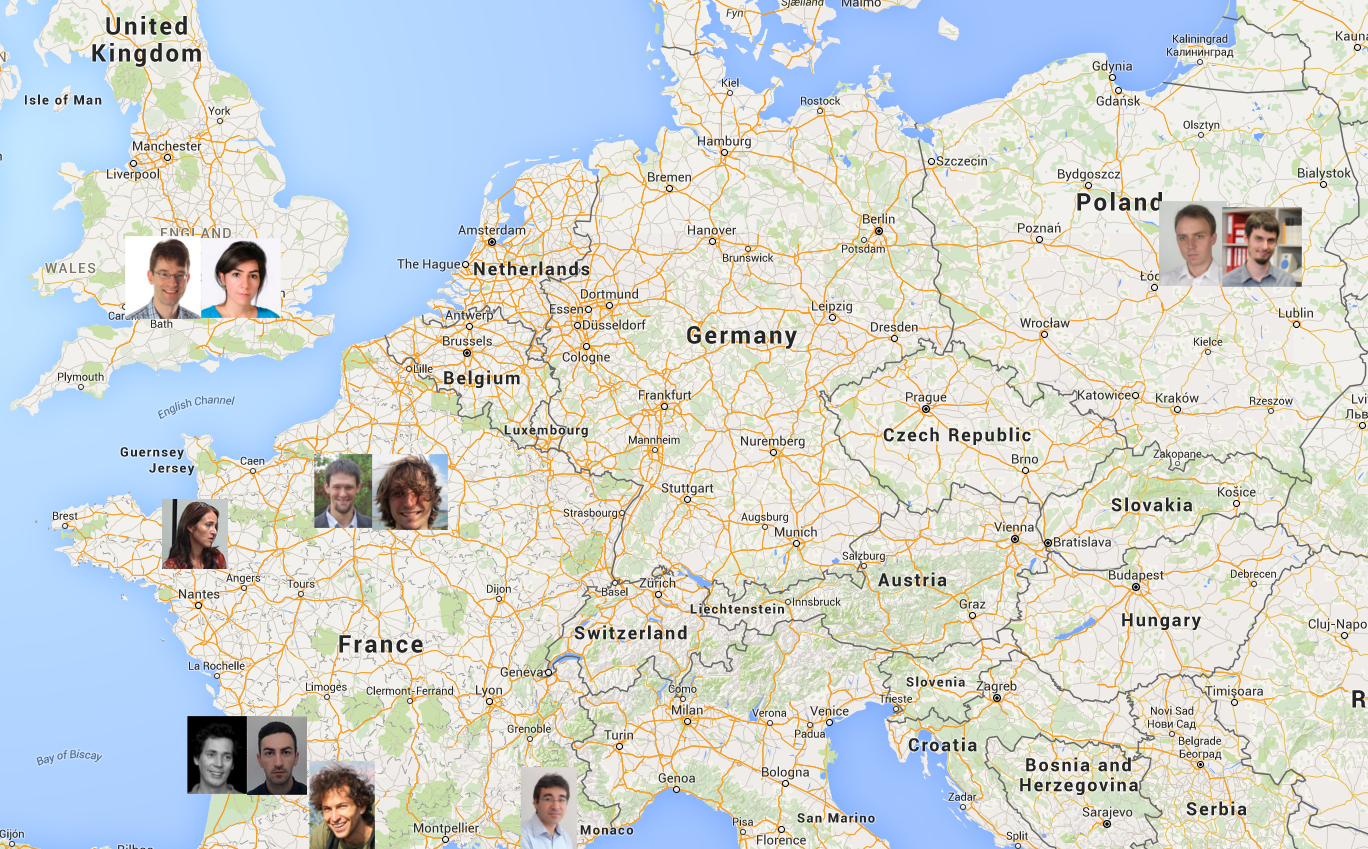
\includegraphics[width=11cm]{Fig/Europe_collaborations}
\end{frame}

\begin{frame}{Activit{\'e} de recherche}

Cadre g{\'e}n{\'e}ral : \textbf{synth{\`e}se de contr{\^o}leur} 

\only<1>{
\begin{center}

\includegraphics[height=2.5cm]{Fig/system}
\hspace*{1cm}

\includegraphics[height=2.5cm]{Fig/formula}
\end{center}
}
\only<2,3,4>{
\begin{center}
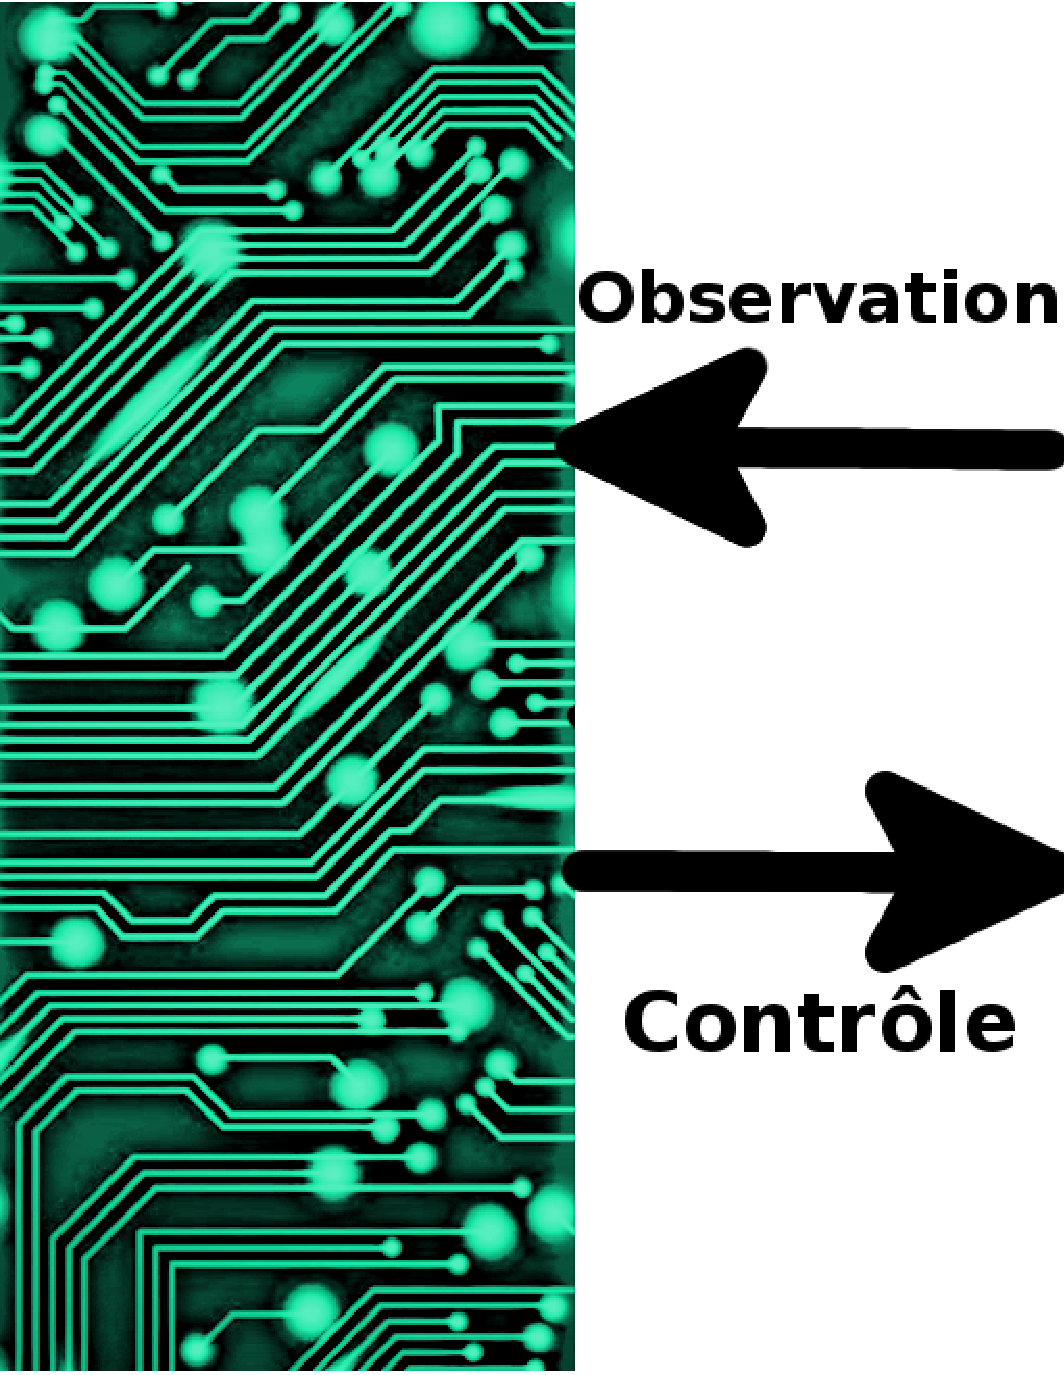
\includegraphics[height=2.5cm]{Fig/controller}

\includegraphics[height=2.5cm]{Fig/system}
\hspace*{1cm}

\includegraphics[height=2.5cm]{Fig/formula}
\end{center}
}

\pause\pause
\vskip1em
Deux aspects :
\begin{enumerate}
	\item[1.] Syst{\`e}mes {\`a} compteurs
	\item[2.] Syst{\`e}mes probabilistes
\end{enumerate}

\vskip1em
\pause
\textit{Outils} : th{\'e}orie des automates, logique, th{\'e}orie des jeux, complexit{\'e}, topologie, alg{\`e}bre...
\end{frame}

\begin{frame}{1. Syst{\`e}mes {\`a} compteurs}
\begin{center}
Conjecture \textcolor{blue}{Colcombet et L{\"o}ding (2010)} :\\
il existe un contr{\^o}leur permettant d'atteindre l'objectif \\
\textcolor{red}{sans consulter la valeur du compteur}.

\begin{picture}(120,28)(-10,5)
	\gasset{Nh=3,Nw=3,Nadjust=wh}

	\node[Nmarks=i,iangle=180](v_9)(0,20){$9$}
	\node(v_8)(10,20){$8$}
	\node(v_7)(20,20){$7$}
	\node(v_6)(30,20){$6$}
	\node(v_5)(40,20){$5$}
	\node(v_4)(50,20){$4$}
	\node(v_3)(60,20){$3$}
	\node(v_2)(70,20){$2$}
	\node(v_1)(80,20){$1$}
	\node(v_0)(90,20){$0$}

	\node(F)(100,20){$F$}

	\drawloop[loopangle=0,loopdiam=3](F){}

	\gasset{curvedepth=-10,linecolor=Blue}

	\drawedge(v_9,v_8){}
	\drawedge(v_8,v_7){}
	\drawedge(v_7,v_6){}
	\drawedge(v_6,v_5){}
	\drawedge(v_5,v_4){}
	\drawedge(v_4,v_3){}
	\drawedge(v_3,v_2){}
	\drawedge(v_2,v_1){}
	\drawedge(v_1,v_0){}
	\drawedge(v_0,F){}
	
	\gasset{linecolor=Purple}

	\drawqbpedge(v_7,130,v_9,80){$r$}
	\drawqbpedge(v_6,130,v_8,80){$r$}
	\drawqbpedge(v_5,130,v_7,80){$r$}
	\drawqbpedge(v_4,130,v_6,80){$r$}
	\drawqbpedge(v_3,130,v_5,80){$r$}
	\drawqbpedge(v_2,130,v_4,80){$r$}
	\drawqbpedge(v_1,130,v_3,80){$r$}
	\drawqbpedge(v_0,130,v_2,80){$r$}

	\gasset{linecolor=Black,linewidth=0.5}

\only<2>{
	\node[fillcolor=Red](token)(0,20){}
	\put(0,2.5){niveau d'{\'e}nergie $3$}
	}

\only<3>{
	\drawedge[linecolor=Red](v_9,v_8){}
	\node[fillcolor=Red](token)(10,20){}
	\put(0,2.5){niveau d'{\'e}nergie $2$}
	}

\only<4>{
	\drawedge[linecolor=Red](v_8,v_7){}
	\node[fillcolor=Red](token)(20,20){}
	\put(0,2.5){niveau d'{\'e}nergie $1$}
	}

\only<5>{
	\drawedge[linecolor=Red](v_7,v_6){}
	\node[fillcolor=Red](token)(30,20){}
	\put(0,2.5){niveau d'{\'e}nergie $0$}
	}

\only<6>{
	\drawqbpedge[linecolor=Red](v_6,130,v_8,80){\textcolor{red}{$r$}}
	\node[fillcolor=Red](token)(10,20){}
	\put(0,2.5){niveau d'{\'e}nergie $3$}
	}
\end{picture}
\end{center}

%\begin{itemize}
%%	\item objectif : case $F$,
%	\item traverser une ar{\^e}te bleue incr{\'e}mente le compteur,
%	\item se d{\'e}placer vers la gauche permet de remettre le compteur {\`a} $0$.
%\end{itemize}

\begin{framed}
\begin{itemize}
	\item Nouveaux outils topologiques donnant des r{\'e}sultats g{\'e}n{\'e}riques,
	\item Contre-exemple {\`a} la conjecture,
	\item Preuve de la conjecture pour des cas particuliers.
\end{itemize}
\end{framed}

\end{frame}

\begin{frame}{Principaux r{\'e}sultats sur les syst{\`e}mes {\`a} compteurs}

\textbf{Construction d'algorithmes pour la synth{\`e}se} :
\begin{itemize}
%	\item Jeux de parit{\'e} et de Streett avec co{\^u}ts [F., Zimmermann, \textsl{FSTTCS'2012}, \textsl{LMCS'2014}]
%	\item Jeux infinis avec conditions finitaires [Chatterjee, F., \textsl{CSL'2013}]
	\item Jeux finis [F., Zimmermann, \textsl{FSTTCS'2012}, \textsl{LMCS'2014}]
	\item Jeux infinis [Chatterjee, F., \textsl{CSL'2013}]
\end{itemize}

\vskip1em
\textbf{Complexit{\'e} des strat{\'e}gies} :
\begin{itemize}
	\item Jeux avec conditions topologiquement closes [Colcombet, F., Horn, \textsl{FSTTCS'2014}]
	\item \textcolor{red}{Compromis entre borne et m{\'e}moire [F., Horn, Kuperberg, Skrzypczak, \textsl{ICALP'2015}]}
\end{itemize}

\vskip1em
\textbf{Impl{\'e}mentation} :
\begin{itemize}
	\item \textcolor{blue}{ACME} [F., Kuperberg, \textsl{ATVA'2014}], \textcolor{blue}{ACME++} [F., Gimbert, Kelmendi, Kuperberg]
\end{itemize}
\end{frame}

\begin{frame}{2. Syst{\`e}mes probabilistes {\`a} information partielle}
\textcolor{blue}{Rabin (63), Bertoni (71), Paz (73), Gimbert et Oualhadj (2010)} :
\begin{center}
Existe t-il un contr{\^o}leur pour atteindre l'objectif \\
\textcolor{red}{avec forte probabilit{\'e}} ?\\

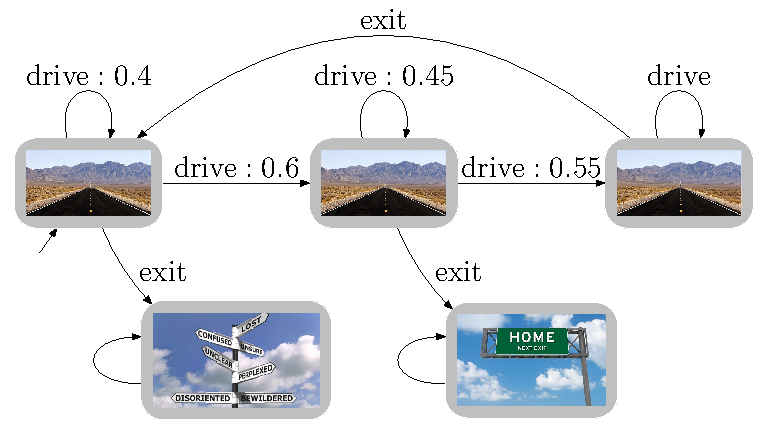
\includegraphics[width=6cm]{Fig/pa}
\end{center}

%\begin{itemize}
%	\item pas de contr{\^o}leur pour rentrer {\`a} la maison \textcolor{blue}{de mani{\`e}re s{\^u}re},
%	\item il existe un contr{\^o}leur pour rentrer {\`a} la maison \textcolor{blue}{avec forte probabilit{\'e}}.
%\end{itemize}

\begin{framed}
\begin{itemize}
	\item Construction d'un algorithme, le meilleur {\`a} ce jour, bas{\'e} sur des techniques alg{\'e}briques,
	\item {\'E}tude avec des outils topologiques.
\end{itemize}
\end{framed}

\end{frame}

\begin{frame}{Principaux r{\'e}sultats sur les syst{\`e}mes probabilistes}

\textbf{Probl{\`e}me de la valeur 1 pour les automates probabilistes} :
\begin{itemize}
	\item \textcolor{red}{Algorithme alg{\'e}brique de Markov [F., Gimbert, Oualhadj, \textsl{LICS'2012}, + Kelmendi, \textsl{LMCS'2015}]}
	\item Perturbations [F., Gimbert, Horn, Oualhadj, \textsl{MFCS'2014}]
	\item \textcolor{red}{Caract{\'e}risation topologique de l'algorithme de Markov [F., \textsl{STACS'2016}]}
\end{itemize}

\vskip1em
\textbf{Simulation de syst{\`e}mes probabilistes} :
\begin{itemize}
	\item ~[F., Pinchinat, Serre, \textsl{FSTTCS'2013}]
	\item ~[F., \textsl{LFCS'2016}]
	\item ~[F., Kiefer, Shirmohammadi, \textsl{FoSSaCS'2016}]
\end{itemize}

\vskip1em
\textbf{Impl{\'e}mentation} :
\begin{itemize}
	\item \textcolor{blue}{ACME} [F., Kuperberg, \textsl{ATVA'2014}], \textcolor{blue}{ACME++} [F., Gimbert, Kelmendi, Kuperberg]
\end{itemize}
\end{frame}

\begin{frame}{Mon projet de recherche}

Deux lignes directrices :
\begin{itemize}
	\item[1.] Approximation des syst{\`e}mes probabilistes
	\item[2.] Complexit{\'e} spatiale en ligne
\end{itemize}
\end{frame}

\begin{frame}{1. Approximation des syst{\`e}mes probabilistes}

\begin{minipage}[b]{0.45\linewidth}
Notion d'approximation :
\begin{itemize}
	\item peu {\'e}tudi{\'e}e en m{\'e}thodes formelles,
	\item naturelle pour \textcolor{red}{mod{\'e}liser},
	\item naturelle pour \textcolor{red}{sp{\'e}cifier},
	\item permet de contourner l'ind{\'e}cidabilit{\'e}.
\end{itemize}
\end{minipage}
\begin{minipage}[b]{0.45\linewidth}
\centering
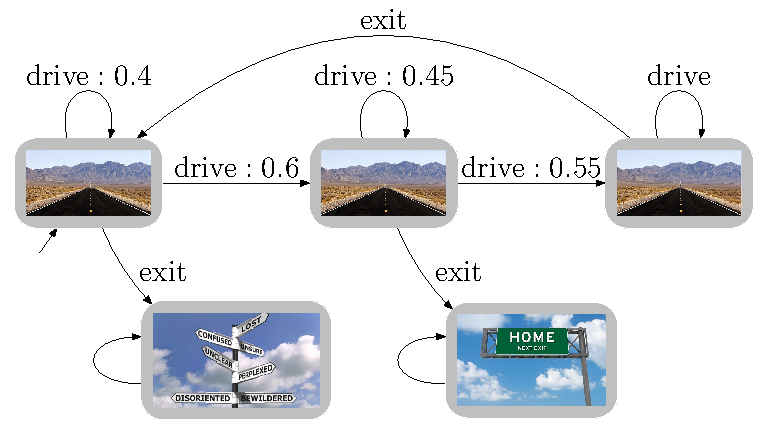
\includegraphics[width=6cm]{Fig/pa}
\end{minipage}

\pause
\vskip1em
\textbf{Objectifs} :
\begin{itemize}
	\item {\`A} moyen terme : analyser les automates probabilistes \textcolor{red}{{\`a} perturbations pr{\`e}s} (\textit{th{\'e}or{\`e}mes d'ergodicit{\'e}}), {\'e}tudier les distances entre syst{\`e}mes probabilistes (\textit{approximation de simulations}),
	\item {\`A} long terme :	d{\'e}velopper une th{\'e}orie math{\'e}matique des syst{\`e}mes al{\'e}atoires \textcolor{red}{{\`a} approximation pr{\`e}s}.
\end{itemize}
\end{frame}

\begin{frame}{2. Complexit{\'e} spatiale en ligne}
\textcolor{blue}{Rabin (1963)} : comment \textcolor{red}{simuler} un automate probabiliste ?

\begin{picture}(80,21)(-2,0)
	\gasset{Nw=6,Nh=6}

  	\node[Nmarks=i,iangle=180](0)(7,5){$1$}
  	\node[Nmarks=r](1)(27,5){$2$}

  	\drawedge(0,1){$a,.6$}
	\drawloop(0){$a,.4$}
	\drawloop(1){$a$}

\Large
\only<2>{
	\put(50,12){$a$}
	\put(50,5){$.6$}
	}

\only<3>{
	\put(50,12){$aa$}
	\put(50,5){$.84$}
	}

\only<4>{
	\put(50,12){$aaa$}
	\put(50,5){$.936$}
	}

\only<5>{
	\put(50,12){$aaaa$}
	\put(50,5){$.9744$}
	}
\end{picture}

\normalsize
\pause\pause\pause\pause
\textcolor{blue}{Karp (1967)} : combien d'\textcolor{red}{espace} est n{\'e}cessaire pour v{\'e}rifier \\
une propri{\'e}t{\'e} \textcolor{red}{en ligne} ?

\vskip1em
\textbf{Objectifs} :
\begin{itemize}
	\item {\`A} moyen terme : classification des automates probabilistes (\textit{th{\'e}or{\`e}mes de d{\'e}composition-s{\'e}paration}), {\'e}tude des automates alternants (\textit{approche logique}),
	\item {\`A} long terme :	m{\'e}thodes de bornes inf{\'e}rieures (\textit{techniques alg{\'e}briques, complexit{\'e} de la communication}), d{\'e}veloppement d'algorithmes g{\'e}n{\'e}riques.
\end{itemize}

%\begin{itemize}
%	\item Propri{\'e}t{\'e}s d{\'e}crites par un automate probabiliste.
%	\item Propri{\'e}t{\'e}s XML.
%\end{itemize}
\end{frame}

\begin{frame}{Int{\'e}gration}
\begin{itemize}
	\item \textcolor{red}{IRISA}, Rennes ({\'e}quipe SUMO)
	\begin{itemize}
		\item Syst{\`e}mes probabilistes : Nathalie Bertrand, Blaise Genest, Ocan Sankur (ANR \textbf{STOCH-MC}), 
		\item Th{\'e}orie du contr{\^o}le : {\'E}ric Fabre, Herv{\'e} Marchand,
		\item V{\'e}rification : Sophie Pinchinat (LOGICA).
	\end{itemize}
	
	\vskip1em
	\item \textcolor{red}{LaBRI}, Bordeaux ({\'e}quipe M{\'e}thodes Formelles)
	\begin{itemize}
		\item Syst{\`e}mes probabilistes : Hugo Gimbert (ANR \textbf{STOCH-MC}), 
		\item Streaming : Olivier Gauwin,
		\item et {\'e}galement J{\'e}r{\^o}me Leroux, Anca Muscholl, Thomas Place, Gabriele Puppis, Igor Walukiewicz, Marc Zeitoun.
	\end{itemize}

	\vskip1em
	\item \textcolor{red}{LIF}, Marseille ({\'e}quipe MOVE)
	\begin{itemize}
		\item V{\'e}rification, Streaming : Pierre-Alain Reynier, Jean-Marc Talbot,
		\item Syst{\`e}mes probabilistes : Benjamin Monm{\`e}ge,
		\item et {\'e}galement Luigi Santocanale.
	\end{itemize}

\end{itemize}

\end{frame}

\begin{frame}{R{\'e}sum{\'e}}
Mon projet de recherche : \textbf{approximation des syst{\`e}mes probabilistes} et \textbf{complexit{\'e} spatiale en ligne}

\vskip1em
\textit{Mots-cl{\'e}s} : syst{\`e}mes al{\'e}atoires, th{\'e}orie des automates, th{\'e}orie des jeux, logique, v{\'e}rification, complexit{\'e}.

\vskip1em
Implication dans la communaut{\'e} scientifique :
\begin{itemize}
\footnotesize
	\item \textcolor{red}{Publications} : 15 conf{\'e}rences, 3 journaux (+ soumissions),
	\item Co-encadrement \textcolor{red}{d'{\'e}tudiants} : Paris (Laureline Pinault, L3), Varsovie (Magdalena Bojarska, M2),
	\item \textcolor{red}{Projets de recherche} : ANR (\textbf{FREC} et \textbf{STOCH-MC}), ERC (\textbf{SOSNA}, \textbf{GALE} et \textbf{AVS-ISS}),
	\item Organisation \textcolor{red}{d'{\'e}v{\`e}nements scientifiques} : s{\'e}minaires (Paris et Oxford), conf{\'e}rences (Highlights) et workshops (GT-\textbf{ALGA}),
	\item D{\'e}veloppement \textcolor{red}{logiciel} (ACME, ACME++, Flides),
	\item Expos{\'e}s \textcolor{red}{invit{\'e}s} (AutoMathA, Cassting). 
\end{itemize}

\normalsize
Diffusion scientifique :
\begin{itemize}
\footnotesize
	\item Responsable de \textcolor{red}{projets Animath} (Kosovo, Laos),
	\item Articles de \textcolor{red}{vulgarisation} (RMS).
\end{itemize}
\end{frame}

\end{document}
